\section*{Введение}
По данным <<Анализа рынка гостиничных услуг в России>>, подготовленного агенством BusinesStat, занимающимся исследованием рынка Российской Федерации и всех стран бывшего СНГ, подобным сервисом в 2022 году воспользовались 62.4 млн чел, что на 63\% превысило значение 2020 года (38.3 млн человек). Такой рост объясняется сокращением выездного туризма и развитием внутреннего на фоне геополитической обстановки. Также численность гостиничных учреждений к концу 2022 года достигла 22.01 тыс., в то время как в 2020 она составляла 20.41 тыс. 

Ввиду сильной конкуренции для привлечения клиентов каждая компания стремится улучшить свой сервис, особое внимание уделяется системам бронирования.

Данное техническое задание определяет требования к разработке распределённой системы бронирования номеров гостиниц сети Apartlux. В неё входят 14 гостиниц в Москве на таких станциях метро, как Бабушкинская, Рижская, Тверская, Авиамоторная и другие.

\section*{Глоссарий}
\begin{enumerate}
	\item REST (Representational State Transfer) -- архитектурный стиль взаимодействия компонентов распределённого приложения в сети. 
	\item ПО -- программное обеспечение.
\end{enumerate}

\section*{Основания для разработки}
Разработка ведётся в рамках выполнения лабораторных работ по курсу <<Методология программной инженерии>> на кафедре <<Программное обеспечение ЭВМ и информационные технологии>> факультета <<Информатика и системы управления>> МГТУ им. Н.Э. Баумана.

\section*{Назначение разработки}
Разрабатываемая система должна предоставлять пользователям возможность поиска и бронирования на интересующие даты. Необходимо реализовать поддержку отмены заказа. Также должна быть предусмотрена опция просмотра полной информации по всем гостиницам, входящих в сеть. В зависимости от количества сделанных ранее заказов система лояльности даёт скидку на новые. Система должна обеспечивать пользователю, как клиенту, возможность просмотра информации как по конкретному, так и по всем бронированиям, статусе в программе лояльности, а как администратору -- доступ ко всей информации с возможностью просмотра, внесения и изменения данных.

\section*{Существующие аналоги}
У сети Apartlux уже есть действующий с 2011 года сайт для бронирования, который имеет ряд недостатков. При его создании разработчики придерживались подходам монолитной архитектуры, поэтому сейчас компания столкнулась с такими трудностями, как:
\begin{enumerate}
	\item проблематичность масштабирования;
	
	\item сложность внедрения появившихся технологий, которые используются повсеместно;
	
	\item внесение даже незначительного изменения в функциональность существенно усложняет и замедляет разработку.
\end{enumerate}

В то время как на российском рынке гостиничных услуг появляется всё больше компаний, например, Radisson, Azimut Hotels, Hilton, остановивших свой выбор на микросервисной архитектуре и внедряющих современные технологии: PostgreSQL, MongoDB, Kafka, ELK stack и т.д. У приведённых сетей отелей и гостиниц есть общий недостаток: непрозрачная программа лояльности, которая направлена лишь на ограниченный круг лиц.

По сравнению с существующим сайтом и указанными аналогами разрабатываемый проект должен иметь следующие преимущества:
\begin{enumerate}
	\item в основе должна лежать микросервисная архитектура, решающая сложности с масштабированием, обслуживанием и внесением изменений в функциональность;
	
	\item понятная бонусная программа, ориентированная на каждого из клиентов.
\end{enumerate}

\section*{Описание системы}
Разрабатываемый сервис должен представлять собой распределённую систему для бронирования номеров гостиниц сети Apartlux. Если клиент хочет оформить бронь, ему необходимо зарегистрироваться, указ информацию: фамилия, имя, отчество, дата рождения, номер телефона. В случае, если зарегистрированному ранее пользователю нужно отменить заказ, получить информацию о его бронированиях или статусе в программе лояльности, ему нужно авторизоваться. Для неавторизованных пользователей доступен только просмотр общей информации. 
На рисунке \ref{fig1:image} отображена схема предметной области.
\begin{figure}[h]
	\begin{center}
		{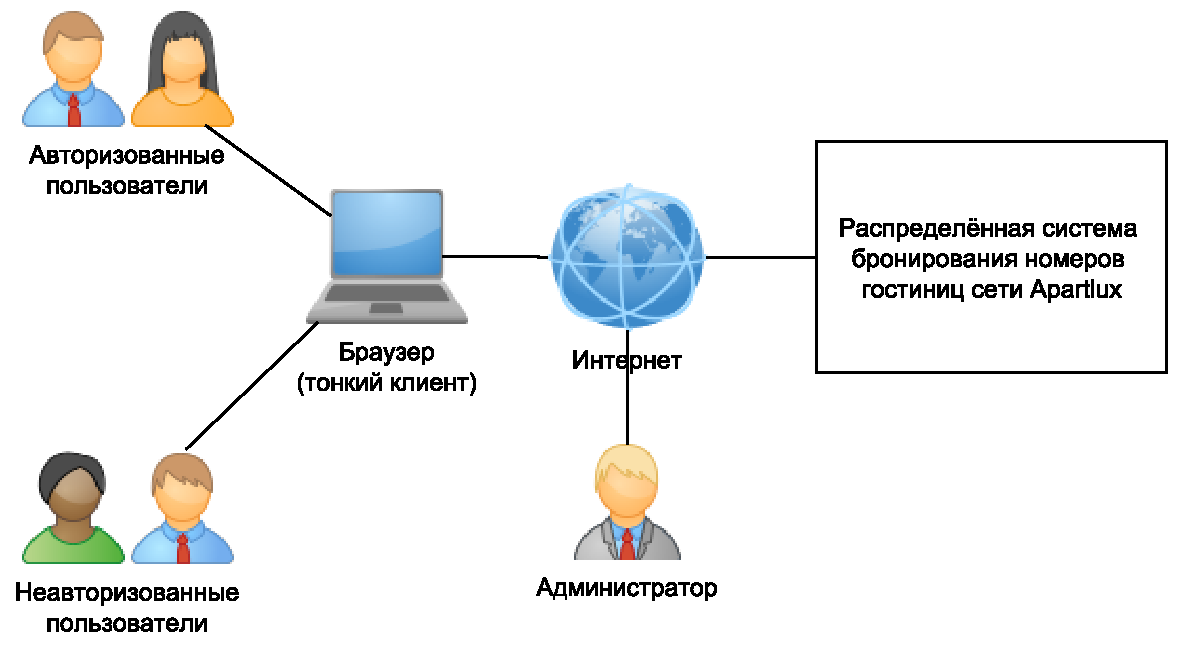
\includegraphics[scale = 0.6]{img/pic/general.pdf}}
		\caption{Схема предметной области.}
		\label{fig1:image}
	\end{center}
\end{figure}

\pagebreak

\section*{Общие требования к системе}
Требования к системе следующие.
\begin{enumerate}
	\item Разрабатываемое ПО должно поддерживать функционирование системы в режиме 24 часов, 7 дней в неделю, 365 дней в году (24/7/365) со среднегодовым временем доступности не менее 99.9\%. Допустимое время, в течении которого система недоступна, за год должна составлять $24\cdot365\cdot0.001=8.76$ ч.
	
	\item Время восстановления системы после сбоя не должно превышать 15 минут.
	
	\item Каждый узел должен автоматически восстанавливаться после сбоя.
	
	\item Система должна поддерживать возможность <<горячего>> переконфигурирования системы. Необходимо предусмотреть поддержку добавления нового узла во время работы системы без рестарта.
	
	\item Обеспечить безопасность работоспособности за счёт отказоустойчивости узлов.
\end{enumerate}

\section*{Требования к функциональным характеристикам}
\begin{enumerate}
	\item По результатам работы модуля сбора статистики медиана времени отклика системы на запросы пользователя на получение информации не должна превышать 3 секунд.
	
	\item По результатам работы модуля сбора статистики медиана времени отклика системы на запросы, добавляющие или изменяющие информацию на портале не должна превышать 7 секунд.
	
	\item Медиана времени отклика системы на действия пользователя должна быть менее 0.8 секунд при условии работы на рекомендованной аппаратной конфигурации, задержках между взаимодействующими сервисами менее 0.2 секунды и одновременном числе работающих пользователей менее 100 на каждый сервер, обслуживающий внешний интерфейс.
	
	\item Система должна обеспечивать возможность запуска в современных браузерах: не менее 85\% пользователей Интернета должны пользоваться ей без какой-либо деградации функционала.
\end{enumerate}

\section*{Функциональные требования к системе с точки зрения пользователя}


 

\pagebreak